\documentclass[10pt]{article}
\usepackage{cite}
\usepackage{graphicx}
\usepackage[hidelinks]{hyperref}
\usepackage[font=small,labelfont=bf]{caption}

% wide margins
\addtolength{\oddsidemargin}{-.75in}
\addtolength{\evensidemargin}{-.75in}
\addtolength{\textwidth}{1.5in}
\addtolength{\topmargin}{-.875in}
\addtolength{\textheight}{1.75in}

\begin{document}

\title{TPL: A Validation System for Secure Peer-to-Peer Exchange}

\author{
  Demian Brener\\
  \texttt{demian@zeppelin.solutions}
  \and
  Santiago Palladino\\
  \texttt{santiago@zeppelin.solutions}
}
\date{March 2018 \\ WORKING DRAFT \\ \small https://tplprotocol.org}
\maketitle
\begin{abstract}

\noindent Participants of an open economy can suffer from scams and immoral activities related to the issuance and exchange of digital assets. Government regulation provides part of the solution, but the main benefits are lost if a trusted third party is required to pass and enforce rules. We propose a solution to prevent malicious behavior by using a self-regulatory framework, elected by a peer-to-peer network and enforced on-chain. Participants in the network delegate trust to authorities for signing certificates and validating their identity in the network. The TPL protocol approves or rejects transactions according to certificate requirements that are coded into digital assets themselves. Any wallet, operating system or exchange (either traditional or decentralized) can automatically adhere to this protocol so that secure connections to other certified participants work seamlessly. In this way, TPL allows any project to guarantee regulatory compliance in every single exchange between participants, and not just in the initial offering. \\

\end{abstract}
\section{Introduction}

Clear guidelines for safe and reliable economic exchange are necessary to prevent malicious behavior within an economy. Scam organizations and theft could be disincentivized by impeding transactions that involve them or blocking electronic payments involving stolen funds. While government regulation works well enough for legacy economic exchange, it suffers from the inherent weakness of having a single party in control of passing, running and enforcing mandatory laws within a jurisdiction. In an inherently decentralized space, the emergence of centralized points of authority is likely to be antagonized.\\

\noindent Territorial-based jurisdictions lack a defined mapping to borderless cryptocurrency spaces. The result for the end user is a multiplicity of regulation sets, not necessarily compatible or consistent with each other, with no clear range of applicability and the uncertainty of change over time. In open exchange platforms, governments conduct their regulatory efforts via proxy - by regulating, auditing, suing and even banning\cite{scmp} centralized exchanges and wallets that hold private keys\cite{coinbase}, or projects selling tokens\cite{zerox}. While aimed at protecting their citizens, tight control and dramatic penalties impose fear. This only ends up reducing the rate of innovation and wealth creation efforts within their jurisdiction.\\

\noindent What is needed is an open regulatory system that is governed by the network and enforced on-chain, allowing parties that trust one another to transact securely. A self-regulatory framework where participation is opt-in allows for the creation of multiple digital jurisdictions, each with its own set of rules, to appeal to different participants while balancing external legal requirements.   \\

\noindent We propose an on-chain protocol for executing digital asset transactions within a peer-to-peer network of trusted participants. A formal decentralized economy creates strong network effects for participants to transact with trusted peers, rather than with participants that haven’t been validated or trusted. \\

\section{Certificates and delegation of trust}

We need a mechanism to ensure the adequate identification of participants according to the regulatory framework elected by the network. The solution we propose borrows from how trusted certificates are used in SSL (Secure Sockets Layer)\cite{digicert}, a protocol created by Netscape in 1994 and adopted by major web browsers to identify secure connections to a server via the Internet\cite{evssl}. \\

\subsection{Governance Collective}

Peer-to-peer networks can be regarded as virtual jurisdictions, not related to geopolitical boundaries, but to different sets of regulations and compliance guarantees. In it, we introduce the concept of a Governance Collective. \\

\noindent A Governance Collective is an entity that governs and manages rules within a jurisdiction. This Governance Collective elects Certificate Validators to attest participant’s identity by signing certificates. Each set of Governance Collective and its approved Certificate Validators represent a jurisdiction with its own set of rules and processes.\\

\begin{figure}[ht]
    \centering
    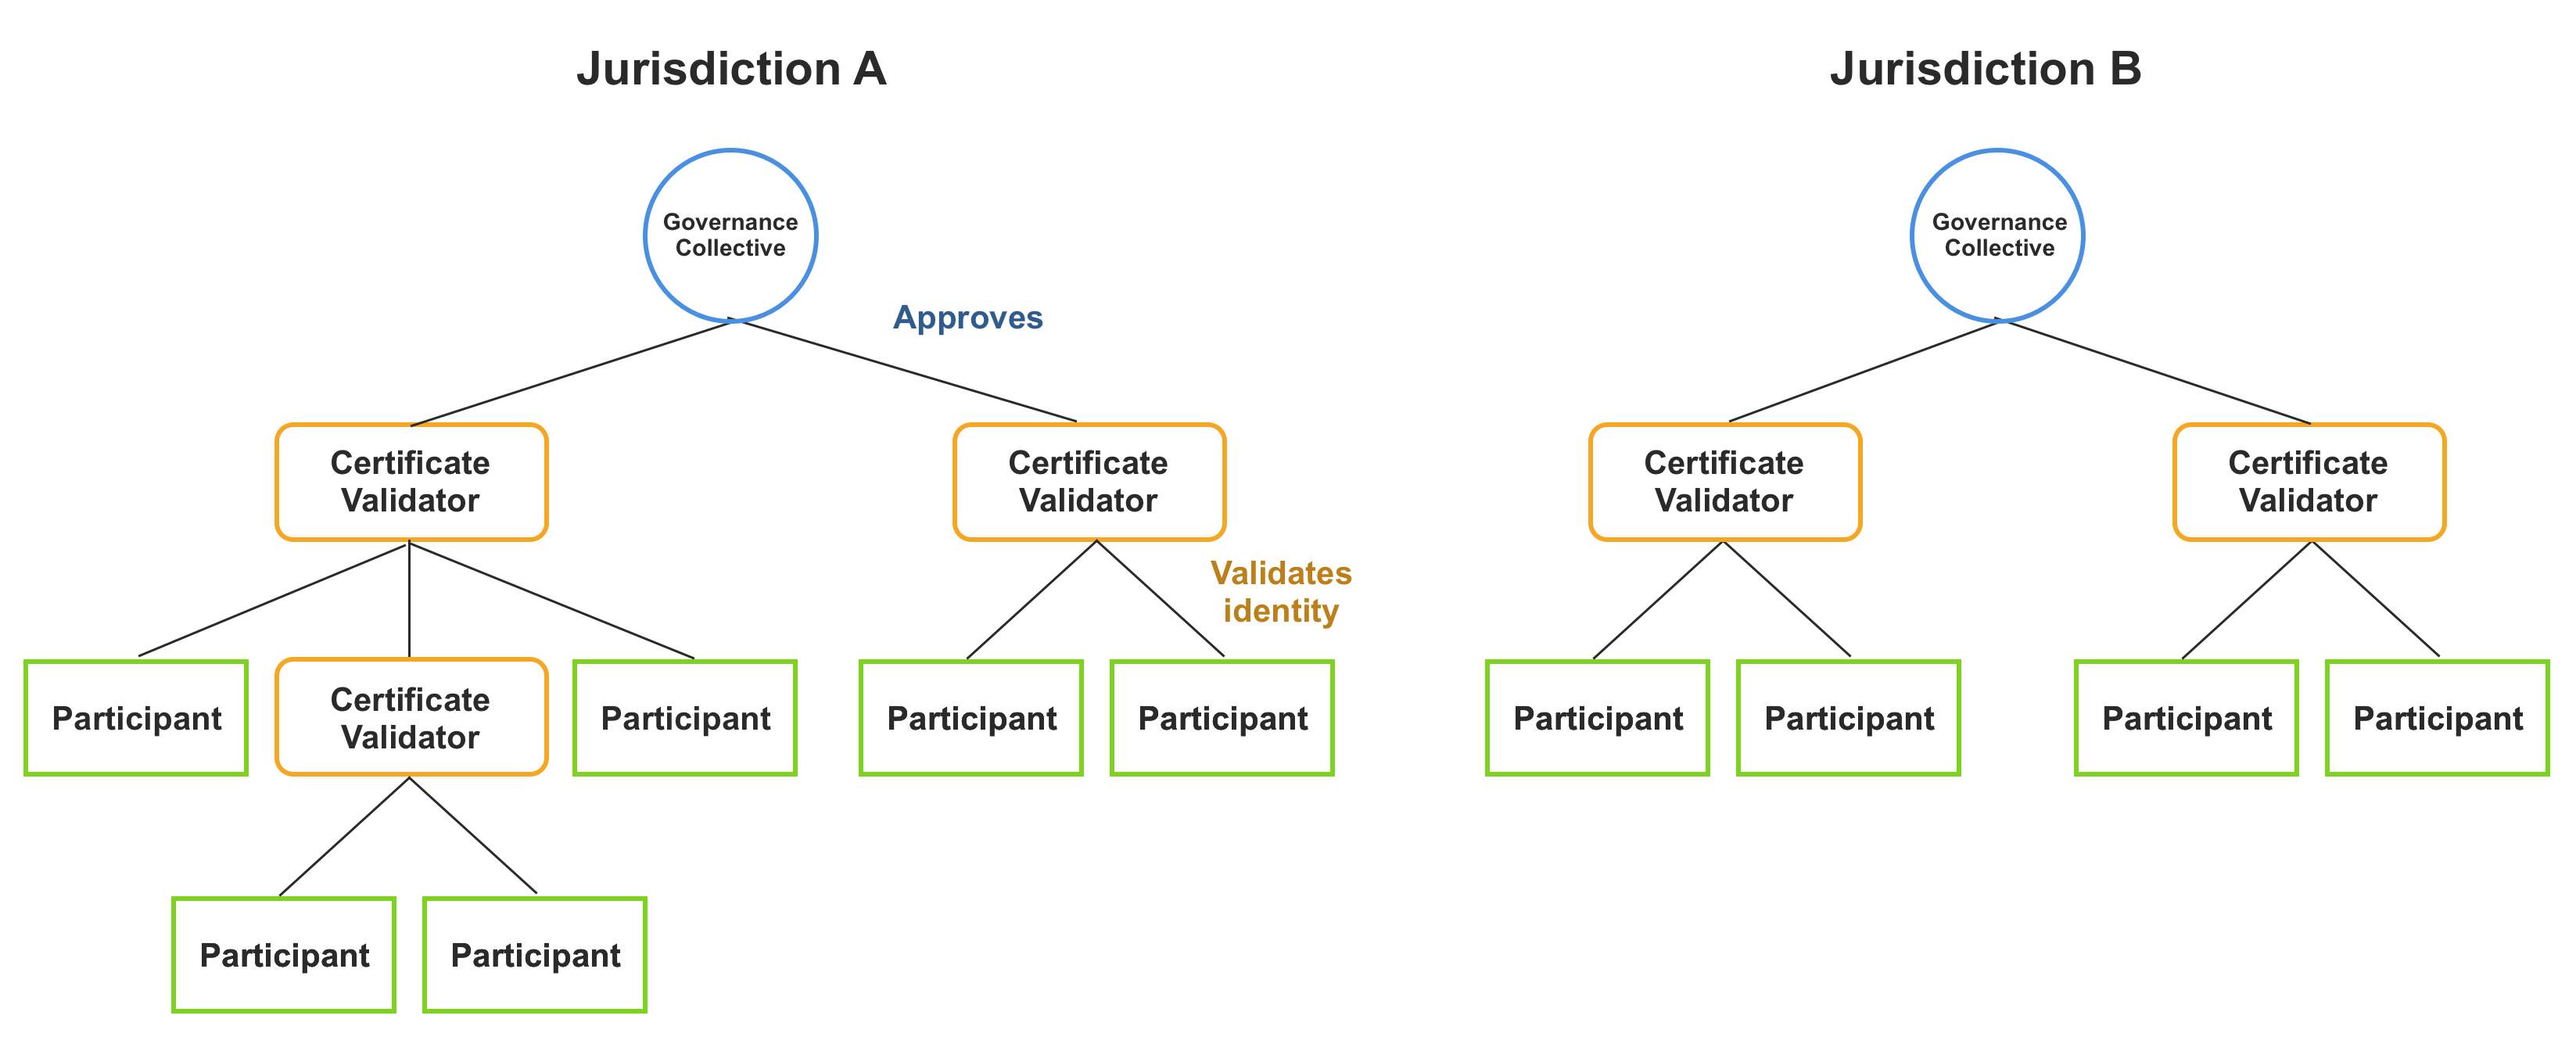
\includegraphics[width=0.8\linewidth]{figures/figure1.png}
    \caption{Delegation of trust between agents of specific jurisdictions, in this case, A and B.}
    \label{fig:fig1}
\end{figure}

\noindent A Governance Collective promulgates industry guidelines governing the issuance and management of certificates within its jurisdiction, analogous to what happens in SSL with a CA/Browser Forum\cite{cabforum}. As a potential Decentralized Autonomous Organization, token holders could govern a Governance Collective following its preferred on-chain governance mechanism\footnote{\ These may range from simple voting to token curated registries for managing lists of approved Certificate Validators.}. \\

\noindent We expect successful Governance Collectives to be set up as a consortium of respected exchanges, wallets, operating systems, and certification validators. These will be trusted organizations from the blockchain space, who can watch over the end-users' interests and balance the legal requirements imposed. The open-source nature of Governance Collectives allows for the creation of multiple jurisdictions to fulfill the needs of different networks. \\

\subsection{Certificate Validator}

A Certificate Validator is a trusted party that performs Know Your Customer (KYC) and Anti Money Laundry (AML) compliance due diligence and investor accreditation to participants in the network. The Governance Collective approves and overlooks the performance of each CV and may oblige them to undergo regular security audits to ensure that they follow all process requirements. The Governance Collective delegates its participants’ trust to CVs for issuing and signing certificates for end users.  \\

\noindent A CV can provide validation services to participants in exchange for a fee (e.g., Verisign\cite{verisign}) or for free (e.g., Let’s Encrypt\cite{letsencrypt}). \\

\noindent CVs may be subject to local governments’ influence, as they perform KYC-AML checks (or any other check required by the Governance Collective) on the off-chain world. CVs have a strong incentive to balance local government pressure with guidelines from the Governance Collective, as it can remove a CV from its trusted set if it deviates from its requirements, instantly revoking all end-user certificates emitted by the entity. \\

\noindent We expect prominent projects within the blockchain space to act as CVs themselves to vouch for their users as part of their service offering. Other projects may fall back to generic CVs who provide such service in exchange for a fee. Additionally, ICO platforms such as Coinlist already perform KYC-AML due diligence and investor accreditation and thus could act as CVs.

\subsection{Participant}

A participant is any individual or entity that wants to transact within a trusted network. Participants rely on certificates to transact with other trusted members. They gain access to these certificates in exchange for sharing their personal data with CVs via KYC-AML procedures. These certificates are valid for a period, after which participants must renew them via CVs. \\

\noindent Participation in a jurisdiction is not exclusive. Participants may have certificates from multiple jurisdictions, should they wish to take part in exchanges in networks with varying requirements. \\

\noindent We expect that the majority of wallets (e.g., MyCryptoWallet), exchanges (e.g., 0x) and operating systems (e.g., ZeppelinOS) will support certificates from various Governance Collectives so that the certificate chain can be validated efficiently, and safe connections to other certified participants work seamlessly.\\

\section{Certificate issuance}
A CV can use a combination of authentication techniques to validate the identity and accreditation of participants. These include leveraging government bureaus, the payment infrastructure, third parties' databases and services, and custom heuristics. \\

\begin{figure}[ht]
    \centering
    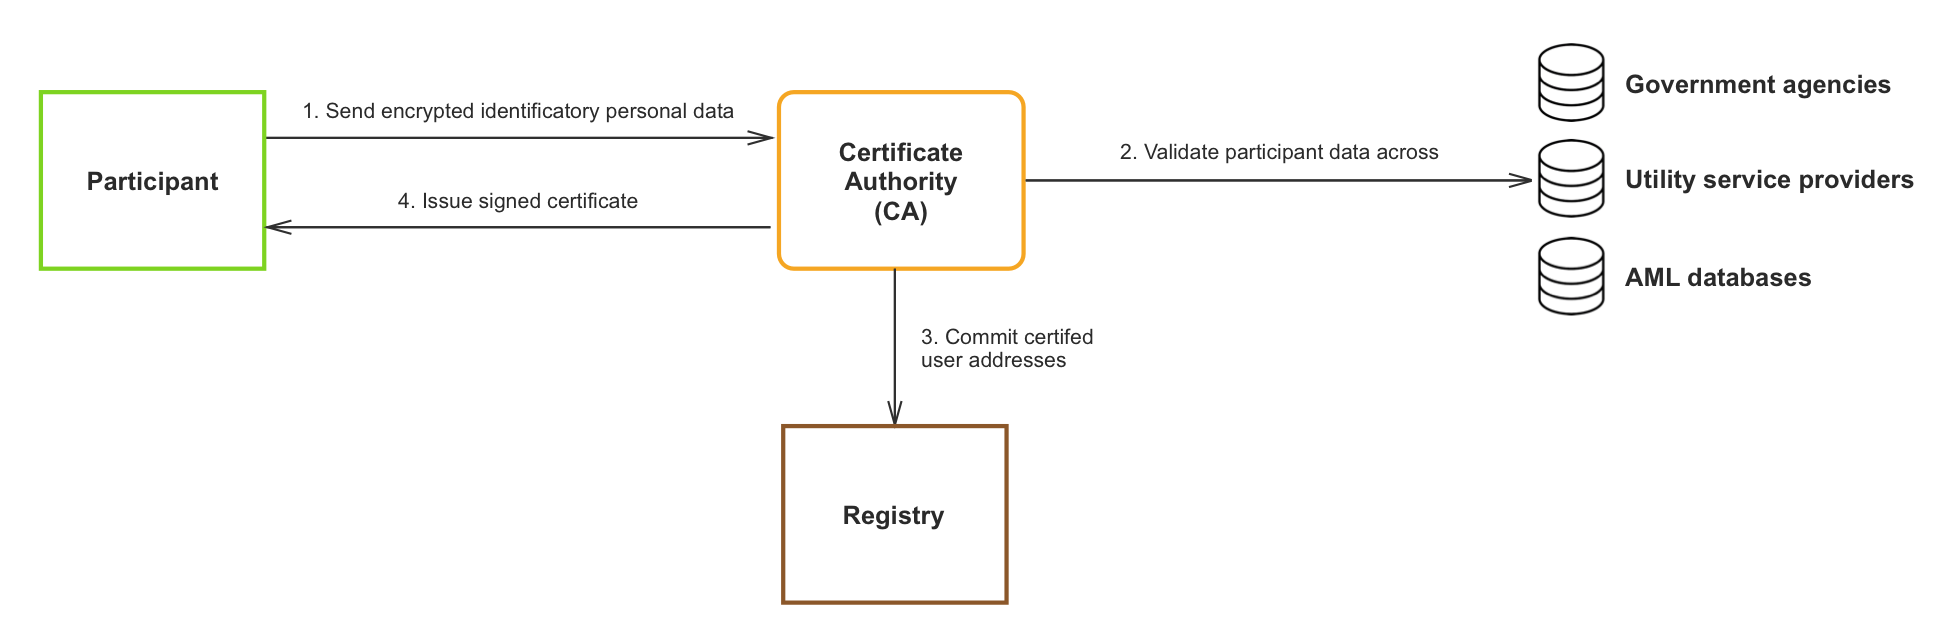
\includegraphics[width=0.8\linewidth]{figures/figure2.png}
    \caption{Validation and certification process.}
    \label{fig:fig2}
\end{figure}

\noindent A CV-issued certificate can include multiple extensions that act as different level authorizations or usage scopes. In the case of an ICO, a project can adhere to a specific jurisdiction, and require participants to hold certificates asserting their accredited investor status and their ability to operate under a particular country’s law\footnote{\ For privacy concerns, the certificate could be used for KYC-AML purposes only without revealing participant’s identity}. Additionally, different certificate extensions could allow for up to a specific volume of transactions.\\

\section{Potential implementations}
Certificates in TPL are analogous to X.509 certificates\cite{x509}, allowing for the re-use of existing tools and libraries to generate and sign certificates.\\

\noindent A Governance Collective signs certificates for the CVs with its private key. CVs then sign the corresponding participants' certificates. When a participant wants to prove that they belong to a jurisdiction, they present the certificate chain up to the Governance Collective certificate.\\

\begin{figure}[ht]
    \centering
    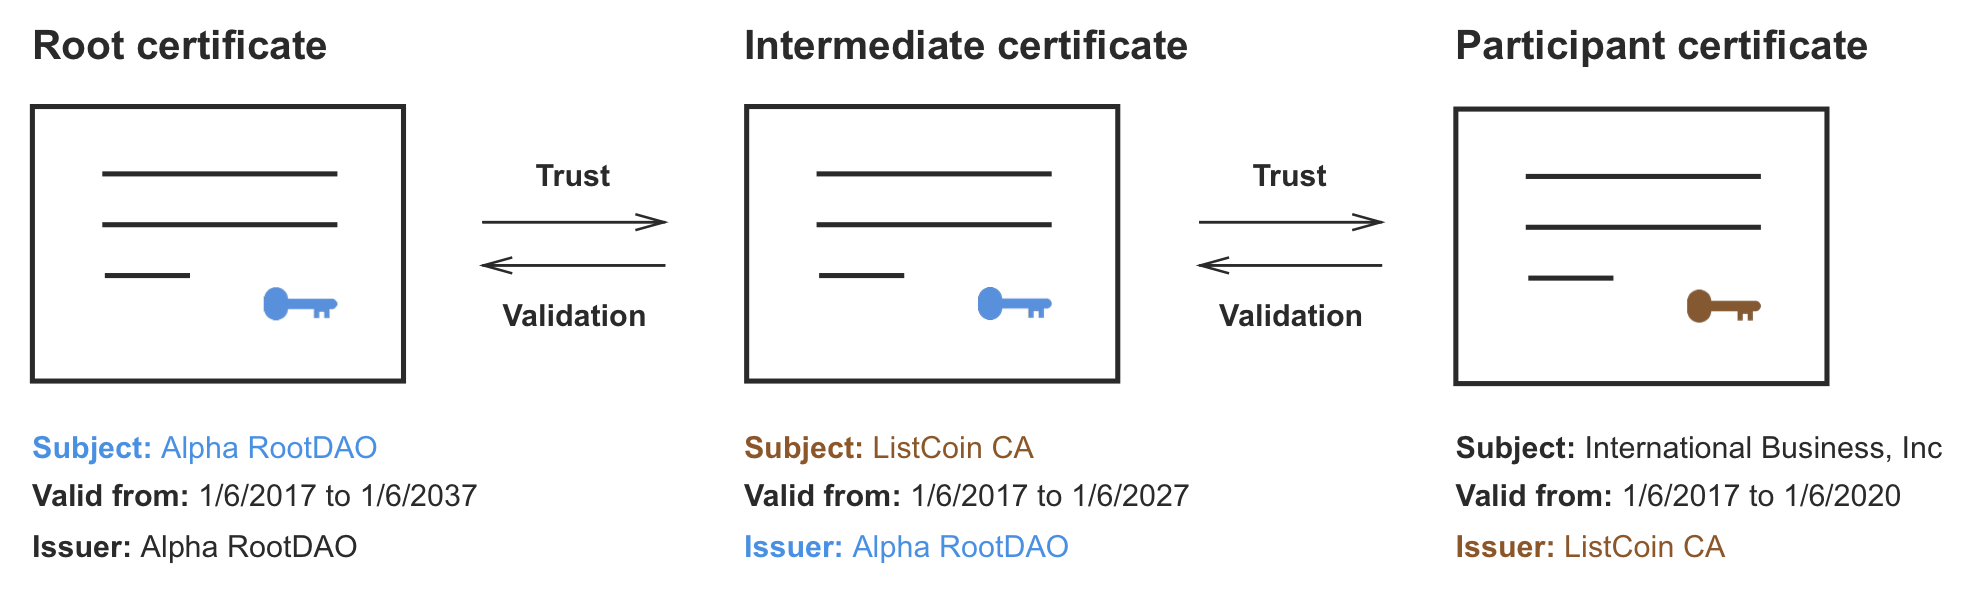
\includegraphics[width=0.8\linewidth]{figures/figure3.png}
    \caption{Validation and certification process.}
    \label{fig:fig3}
\end{figure}

\noindent A Governance Collective governs a smart contract on the Ethereum\cite{ethereum} blockchain that mirrors the chain of trust of certificates. This smart contract-based registry allows any smart contract to easily check that a participant is indeed part of the jurisdiction by querying this on-chain registry, rather than cryptographically verifying the authenticity of the certificate chain. Additionally, having all certificate info in a single smart contract facilitates certificate revocation\footnote{\ This outperforms protocols like CRLs or OCSP}.\\

\subsection{Approval of transactions between trusted participants within a jurisdiction}
The logic for transaction approval can be automated and built-in within the smart contract code of a token or an exchange. TPL can enforce any compliance rule required by a project sponsoring an asset, assuring that all participants in a transaction have been adequately vetted.\\

\noindent This mechanism allows any project to ensure that not only their ICO will be compliant, but also any subsequent transactions of their asset between any third parties since the contract itself can reject any operations from unauthorized users. Different token contracts may demand various extensions to be present from the transaction participants certificates, thus effectively placing on-chain any off-chain compliance requirements. Any vendor (wallet, operating system or exchange, either traditional or decentralized) will automatically adhere to these requirements since they are coded into the digital asset itself.\\

\begin{figure}[ht]
    \centering
    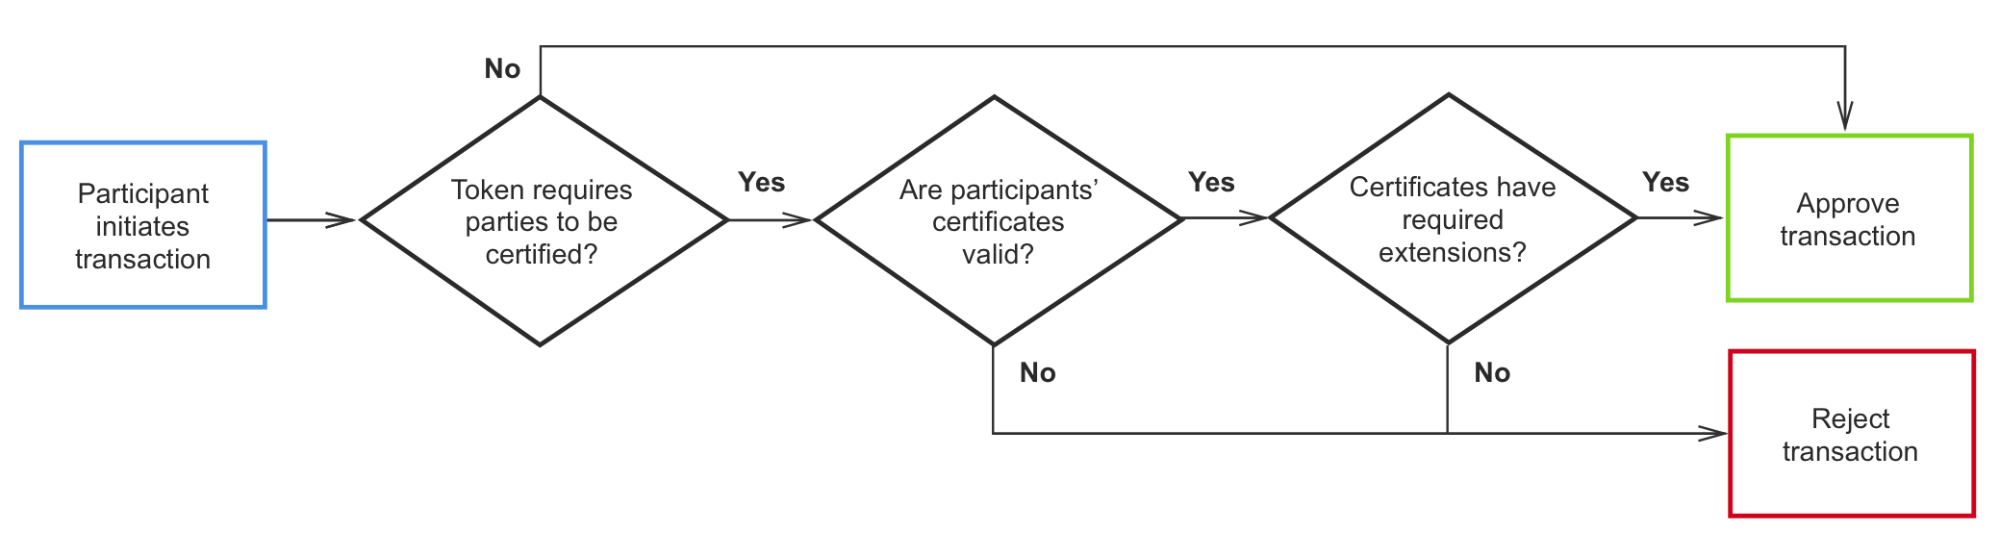
\includegraphics[width=0.8\linewidth]{figures/figure4.png}
    \caption{Validation and certification process.}
    \label{fig:fig4}
\end{figure}

\noindent Alternatively, if TPL is not built-in within an asset smart contract code, any vendor can still protect its end users by querying participants’ certificate identities within the jurisdiction public registry.\\

\section{Next steps}
Blockchain technology empowers the individual, holding the promise of an open financial system. While it has steadily matured over the last few years, significant challenges remain, in particular towards integration with the traditional financial system. If performed wisely, this integration could lead to a new world in which the usual power relations are inverted, and individuals are in control.\\

\noindent This process, however, might be at risk if driven from outside the system as institutions will naturally favor the status quo. To be successful, the integration must be led from within, proposing clear guidelines on how to onboard institutional players. TPL is a first approach in this direction, providing a self-regulatory framework to support formal decentralized economies while preserving users’ freedom to assemble and innovate.\\
 
\noindent Should this idea find consensus among the community, we will include support for permissioned tokens within OpenZeppelin\cite{openzeppelin}, a standard framework of reusable and secure smart contracts in the Solidity language. \\

\bibliography{bib}{}
\bibliographystyle{unsrt}
   
\end{document}
